\documentclass[sigconf]{acmart}

\usepackage{mathptmx}
\usepackage{amsmath}
\usepackage{tikz}
\usepackage{pgfplots}
\usepgfplotslibrary{groupplots}
\usepgfplotslibrary{colorbrewer}
\usepackage{datatool}
\usepackage{ifthen}
% Curly braces
\usetikzlibrary{arrows.meta,decorations.pathreplacing,angles,quotes,patterns}
% Relative positioning
\usetikzlibrary[positioning]

\usepackage[binary-units]{siunitx}
\DeclareSIUnit\dBm{\dB\text{m}}

\tikzset{annotation/.style={scale=0.85,fill=white,inner sep=1,outer sep=3}}
\tikzset{txarrow/.style={-{Latex[scale=1.5]},dashed}}

\makeatletter
\def\pgfplots@stacked@diff{}
\makeatother

\definecolor{inkscape-royalblue}{RGB}{65,105,225}
\definecolor{inkscape-firebrick}{RGB}{178,34,34}
\definecolor{inkscape-forestgreen}{RGB}{85,155,85}
\definecolor{inkscape-khaki}{RGB}{240,230,140}
\definecolor{inkscape-lightsteelblue}{RGB}{176,196,222}

\definecolor{verylightgray}{gray}{0.85}
\definecolor{lightgray}{gray}{0.75}
\definecolor{darkgray}{gray}{0.5}

% x, y, color, prefix for node names, scaling
\newcommand{\tikzdrawframe}[5]{
	\node [draw,fill=white,rectangle,minimum height=4*#5,minimum width=3] (#4_preamble) at (#1,#2) {};
	\node [draw,fill=#3,rectangle,minimum height=10*#5,minimum width=3] (#4_payload) [below=of #4_preamble] {};
}

% x, y, node name
\newcommand{\tikzdrawwindow}[3]{
	\node [draw,dotted,fill=white,rectangle,minimum height=4,minimum width=10] (#3) at (#1,#2) {};
}

% from https://tex.stackexchange.com/a/178632
\pgfplotsset{
	discard if not/.style 2 args={
		x filter/.code={
			\edef\tempa{\thisrow{#1}}
			\edef\tempb{#2}
			\ifx\tempa\tempb
			\else
			\def\pgfmathresult{inf}
			\fi
		}
	}
}

\DeclareSymbolFont{symbolsb}{OMS}{cmsy}{m}{n}
\SetSymbolFont{symbolsb}{bold}{OMS}{cmsy}{b}{n}
\DeclareSymbolFontAlphabet{\mathcal}{symbolsb}


\begin{document}
\begin{minipage}{85mm}
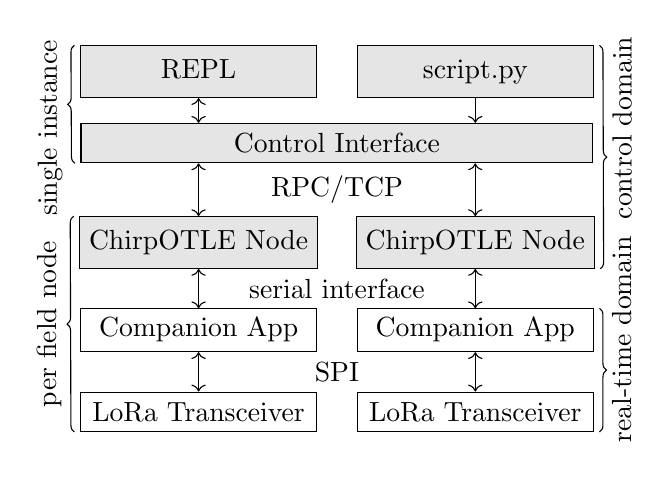
\begin{tikzpicture}
\tikzset{
	block/.style={rectangle,minimum width=3cm,minimum height=.5cm},
	ctrlblock/.style={block,draw=black,fill=gray!20!white},
	rtblock/.style={block,draw=black},
	dblsize/.style={minimum width=6.5cm},
}

\node [ctrlblock] (repl) {\strut{}REPL};
\node [ctrlblock] (script) [right=.5cm of repl] {\strut{}script.py};

\path (repl) -- node [ctrlblock, dblsize] (controlinterface) [below=.65cm] {Control Interface} (script);
\draw [<->] (repl) -- (repl|-controlinterface.north);
\draw [->] (script) -- (script|-controlinterface.north);

\node [ctrlblock] (loranode0) [below=1.5cm of repl] {\strut{}ChirpOTLE Node};
\node [ctrlblock] (loranode1) [below=1.5cm of script] {\strut{}ChirpOTLE Node};
\draw [<->] (loranode0|-controlinterface.south) -- node [right,align=center,minimum width=3.5cm] {RPC/TCP} (loranode0);
\draw [<->] (loranode1|-controlinterface.south) -- (loranode1);

\node[rtblock] (companion0) [below=.5cm of loranode0] {Companion App};
\node[rtblock] (companion1) [below=.5cm of loranode1] {Companion App};
\draw [<->] (loranode0) --  node [right,align=center,minimum width=3.5cm] {serial interface} (companion0);
\draw [<->] (loranode1) --(companion1);

\node[rtblock] (lora0) [below=.5cm of companion0] {LoRa Transceiver};
\node[rtblock] (lora1) [below=.5cm of companion1] {LoRa Transceiver};
\draw[<->] (companion0) --  node [right,align=center,minimum width=3.5cm] {SPI} (lora0);
\draw[<->] (companion1) -- (lora1);

% Right braces: Domains
\draw[decoration={brace,raise=2pt},decorate]  (script.north east) -- node[below,xshift=3pt,rotate=90,pos=.37] {control domain} (loranode1.south east);
\draw[decoration={brace,raise=2pt},decorate]  (companion1.north east) -- node[below,xshift=3pt,rotate=90,pos=0.25] {real-time domain} (lora1.south east);

% Left braces: Location
\draw[decoration={brace,raise=2pt,mirror},decorate]  (repl.north west) -- node[above,xshift=-3pt,rotate=90,pos=.7] {single instance} (controlinterface.south west);
\draw[decoration={brace,raise=2pt,mirror},decorate]  (loranode0.north west) -- node[above,xshift=-3pt,rotate=90] {per field node} (lora0.south west);

\end{tikzpicture}
\end{minipage}
\end{document}
